% =====================================================================
%  VaayuMitra -- IIT Madras Research Scholars' Day 2026 poster (LaTeX)
%  Official RSD template used as a vector background (template_bg.pdf).
%  Compile with XeLaTeX (Overleaf: Menu -> Compiler -> XeLaTeX) or Tectonic.
%  All numbers come from numbers.tex (auto-generated by src/make_latex_numbers.py).
%  One font everywhere: TeX Gyre Termes (fonts/), also used inside every figure.
% =====================================================================
\documentclass{article}
\usepackage[paperwidth=594mm,paperheight=841mm,
            top=5.24in,left=0.6in,right=0.585in,bottom=0.42in]{geometry}
\usepackage{fontspec}
\setmainfont{texgyretermes}[Path=fonts/, Extension=.otf, UprightFont=*-regular, BoldFont=*-bold,
  ItalicFont=*-italic, BoldItalicFont=*-bolditalic]
\usepackage{unicode-math}
\setmathfont{texgyretermes-math.otf}[Path=fonts/]
\usepackage{newunicodechar}
\IfFileExists{tfrupee.sty}{\usepackage{tfrupee}\newunicodechar{₹}{\rupee}}{\newunicodechar{₹}{Rs.\,}}
\newunicodechar{→}{\ensuremath{\rightarrow}}
\newunicodechar{−}{\ensuremath{-}}
\newunicodechar{≈}{\ensuremath{\approx}}
\newunicodechar{✓}{\ensuremath{\checkmark}}
\usepackage{xcolor,graphicx,eso-pic,tikz,amsmath,enumitem,array,booktabs,tabularx,ragged2e,microtype}
\usepackage[most]{tcolorbox}
\usetikzlibrary{arrows.meta,positioning,calc}
% auto-generated by src/make_latex_numbers.py -- do not edit by hand
\newcommand{\NTrips}{2,365,848}
\newcommand{\Span}{Jan 2015--Dec 2024}
\newcommand{\Rsq}{0.988}
\newcommand{\MAE}{0.33}
\newcommand{\Qband}{0.7}
\newcommand{\Cover}{89}
\newcommand{\Payback}{3}
\newcommand{\InrBoat}{52}
\newcommand{\LakhPkg}{2.2}
\newcommand{\MLdiesel}{51}
\newcommand{\Crore}{508}
\newcommand{\Ktco}{136}
\newcommand{\Craft}{97,659}
\newcommand{\East}{21}
\newcommand{\West}{12}
\newcommand{\Tip}{27}
\newcommand{\NCell}{100}
\newcommand{\APcr}{76}
\newcommand{\KLcr}{48}
\newcommand{\Kochi}{8}
\newcommand{\Chennai}{15}
\newcommand{\Vizag}{20}
\newcommand{\BestPct}{29}
\newcommand{\BestMonth}{April}
\newcommand{\PkgBefore}{25}
\newcommand{\PkgAfter}{14}
\newcommand{\PkgPct}{44}
\newcommand{\LiveDay}{16 Nov 2026}
\newcommand{\HabitFuel}{27.9}
\newcommand{\HabitTrip}{12.2}
\newcommand{\SailFuel}{21.8}
\newcommand{\SailHours}{6.2}
\newcommand{\BestDep}{08:00}
\newcommand{\BestSpeed}{7}
\newcommand{\BestSail}{7.1}
\newcommand{\BestFuel}{16.0}
\newcommand{\BestTrip}{13.1}
\newcommand{\BestWind}{7.7}
\newcommand{\BestHs}{1.7}
\newcommand{\BestSaveL}{11.9}
\newcommand{\BestSaveRs}{1,190}
\newcommand{\BestSavePct}{43}
\newcommand{\BaseL}{16.8}
\newcommand{\PayAtSix}{7}
\newcommand{\PayAtTen}{4}
\newcommand{\InrAtSix}{20}
\newcommand{\PayWorst}{8}
\newcommand{\PayMin}{1.8}
\newcommand{\PayMax}{4.6}


% ---------- colours: green theme (template green 055A08) ----------
\definecolor{tg}{HTML}{055A08}\definecolor{dg}{HTML}{0B4D1C}\definecolor{mg}{HTML}{2E8B3E}
\definecolor{lg}{HTML}{ECF6EC}\definecolor{lg2}{HTML}{C9E4CC}
\definecolor{acc}{HTML}{C0392B}\definecolor{ink}{HTML}{1A1A1A}
\definecolor{cblue}{HTML}{2A78D6}\definecolor{corange}{HTML}{EB6834}
\color{ink}

% ---------- type and justification ----------
\renewcommand{\normalsize}{\fontsize{18.5}{22.2}\selectfont}
\newcommand{\capsz}{\fontsize{15}{17.8}\selectfont}
\newcommand{\smallish}{\fontsize{17}{20.5}\selectfont}
\newcommand{\hl}[1]{\textcolor{acc}{\textbf{#1}}}
\newcommand{\gb}[1]{\textcolor{tg}{\textbf{#1}}}
\setlength{\parindent}{0pt}
\emergencystretch=2.5em \tolerance=2000 \hyphenpenalty=200
\setlength{\JustifyingParindent}{0pt}
\let\oldjustifying\justifying   % justified text whose last line is never near-empty (no one-word lines)
\renewcommand{\justifying}{\oldjustifying\parfillskip=0pt plus 0.72\linewidth\relax}
\setlist[itemize]{leftmargin=1.0em,itemsep=3pt,topsep=2pt,parsep=0pt,partopsep=0pt,
  label={\raisebox{0.1ex}{\textcolor{mg}{\large$\circ$}}}, before=\justifying}
\newcounter{fig}
\newcommand{\figcap}[1]{\refstepcounter{fig}{\capsz\justifying\textbf{Figure~\thefig.}~#1\par}}

% ---------- section box (banner title, like the reference) ----------
\newtcolorbox{secbox}[2][]{enhanced, colback=white, colframe=tg, boxrule=0.8mm, arc=6mm,
  left=6mm, right=6mm, top=9mm, bottom=3mm, halign=justify,
  title={#2}, coltitle=white, fonttitle=\fontsize{30}{34}\selectfont\bfseries,
  attach boxed title to top center={yshift=-6mm, yshifttext=-3mm},
  underlay boxed title={\fill[white] ([xshift=-3mm,yshift=-1mm]title.south west) rectangle ([xshift=3mm,yshift=1mm]title.north east);},
  boxed title style={enhanced, colback=tg, colframe=tg, arc=6mm, boxrule=0pt,
                     left=14mm, right=14mm, top=1.5mm, bottom=1.5mm},
  before skip=0pt, after skip=0pt, before upper=\justifying, #1}
\newtcolorbox{tile}[1][]{enhanced, colback=lg, colframe=lg2, boxrule=0.6mm, arc=3mm,
  left=1mm, right=1mm, top=1.5mm, bottom=1.5mm, halign=center, valign=center, before upper=\centering, #1}

% ---------- background (official template) + title in its heading box ----------
\AddToShipoutPictureBG*{
\includegraphics[width=\paperwidth,height=\paperheight]{template_bg.pdf}}
\AddToShipoutPictureFG*{\begin{tikzpicture}[remember picture,overlay]
  \node[anchor=center, text width=15.0in, align=flush center] at ([xshift=11.72in,yshift=-1.66in]current page.north west) {%
    {\fontsize{50}{56}\selectfont\bfseries VaayuMitra: Wind-Smart Sails for Fishing Boats}\\[8pt]
    {\fontsize{24}{28}\selectfont\itshape\color{tg} Forecast-driven sail assistance that cuts diesel, cost and CO$_2$ for India's small-scale fishers}\\[9pt]
    {\fontsize{23}{27}\selectfont [Your Name] \quad\textbullet\quad Department of Ocean Engineering, IIT Madras}};
\end{tikzpicture}}

\newlength{\colH}\setlength{\colH}{18.75in}
\newlength{\padL}\setlength{\padL}{0pt}\newlength{\padR}\setlength{\padR}{28pt}  % = L-R from the COLS line in poster.log
\newlength{\gap}\setlength{\gap}{0.28in}   % equal space between all boxes   % height of the two-column block

\begin{document}\pagestyle{empty}\normalsize
\noindent
% =====================================================================
%  LEFT COLUMN
% =====================================================================
\newsavebox{\lcol}\newsavebox{\rcol}
\sbox{\lcol}{\begin{minipage}[t]{0.493\textwidth}\vspace{0pt}
% ---------------- 1. PROBLEM ----------------
\begin{secbox}{Why Fishers Need the Wind Back}
\begin{minipage}[t]{0.585\linewidth}\vspace{0pt}
\begin{itemize}
  \item \hl{Diesel is the largest cost} for India's small-scale fishers and its price keeps rising; every litre burnt also emits \textbf{2.68\,kg of CO$_2$}.
  \item The \gb{monsoon winds} that once drove Indian sailing craft now blow past these motorised boats unused.
  \item FAO sail trials on Kerala boats (1981--83) worked, yet the sail was up only \hl{10--16\,\% of travel time}, because fishers had \textbf{no way to know when sailing pays} [1].
\end{itemize}
\end{minipage}\hfill
\begin{minipage}[t]{0.39\linewidth}\vspace{2pt}
  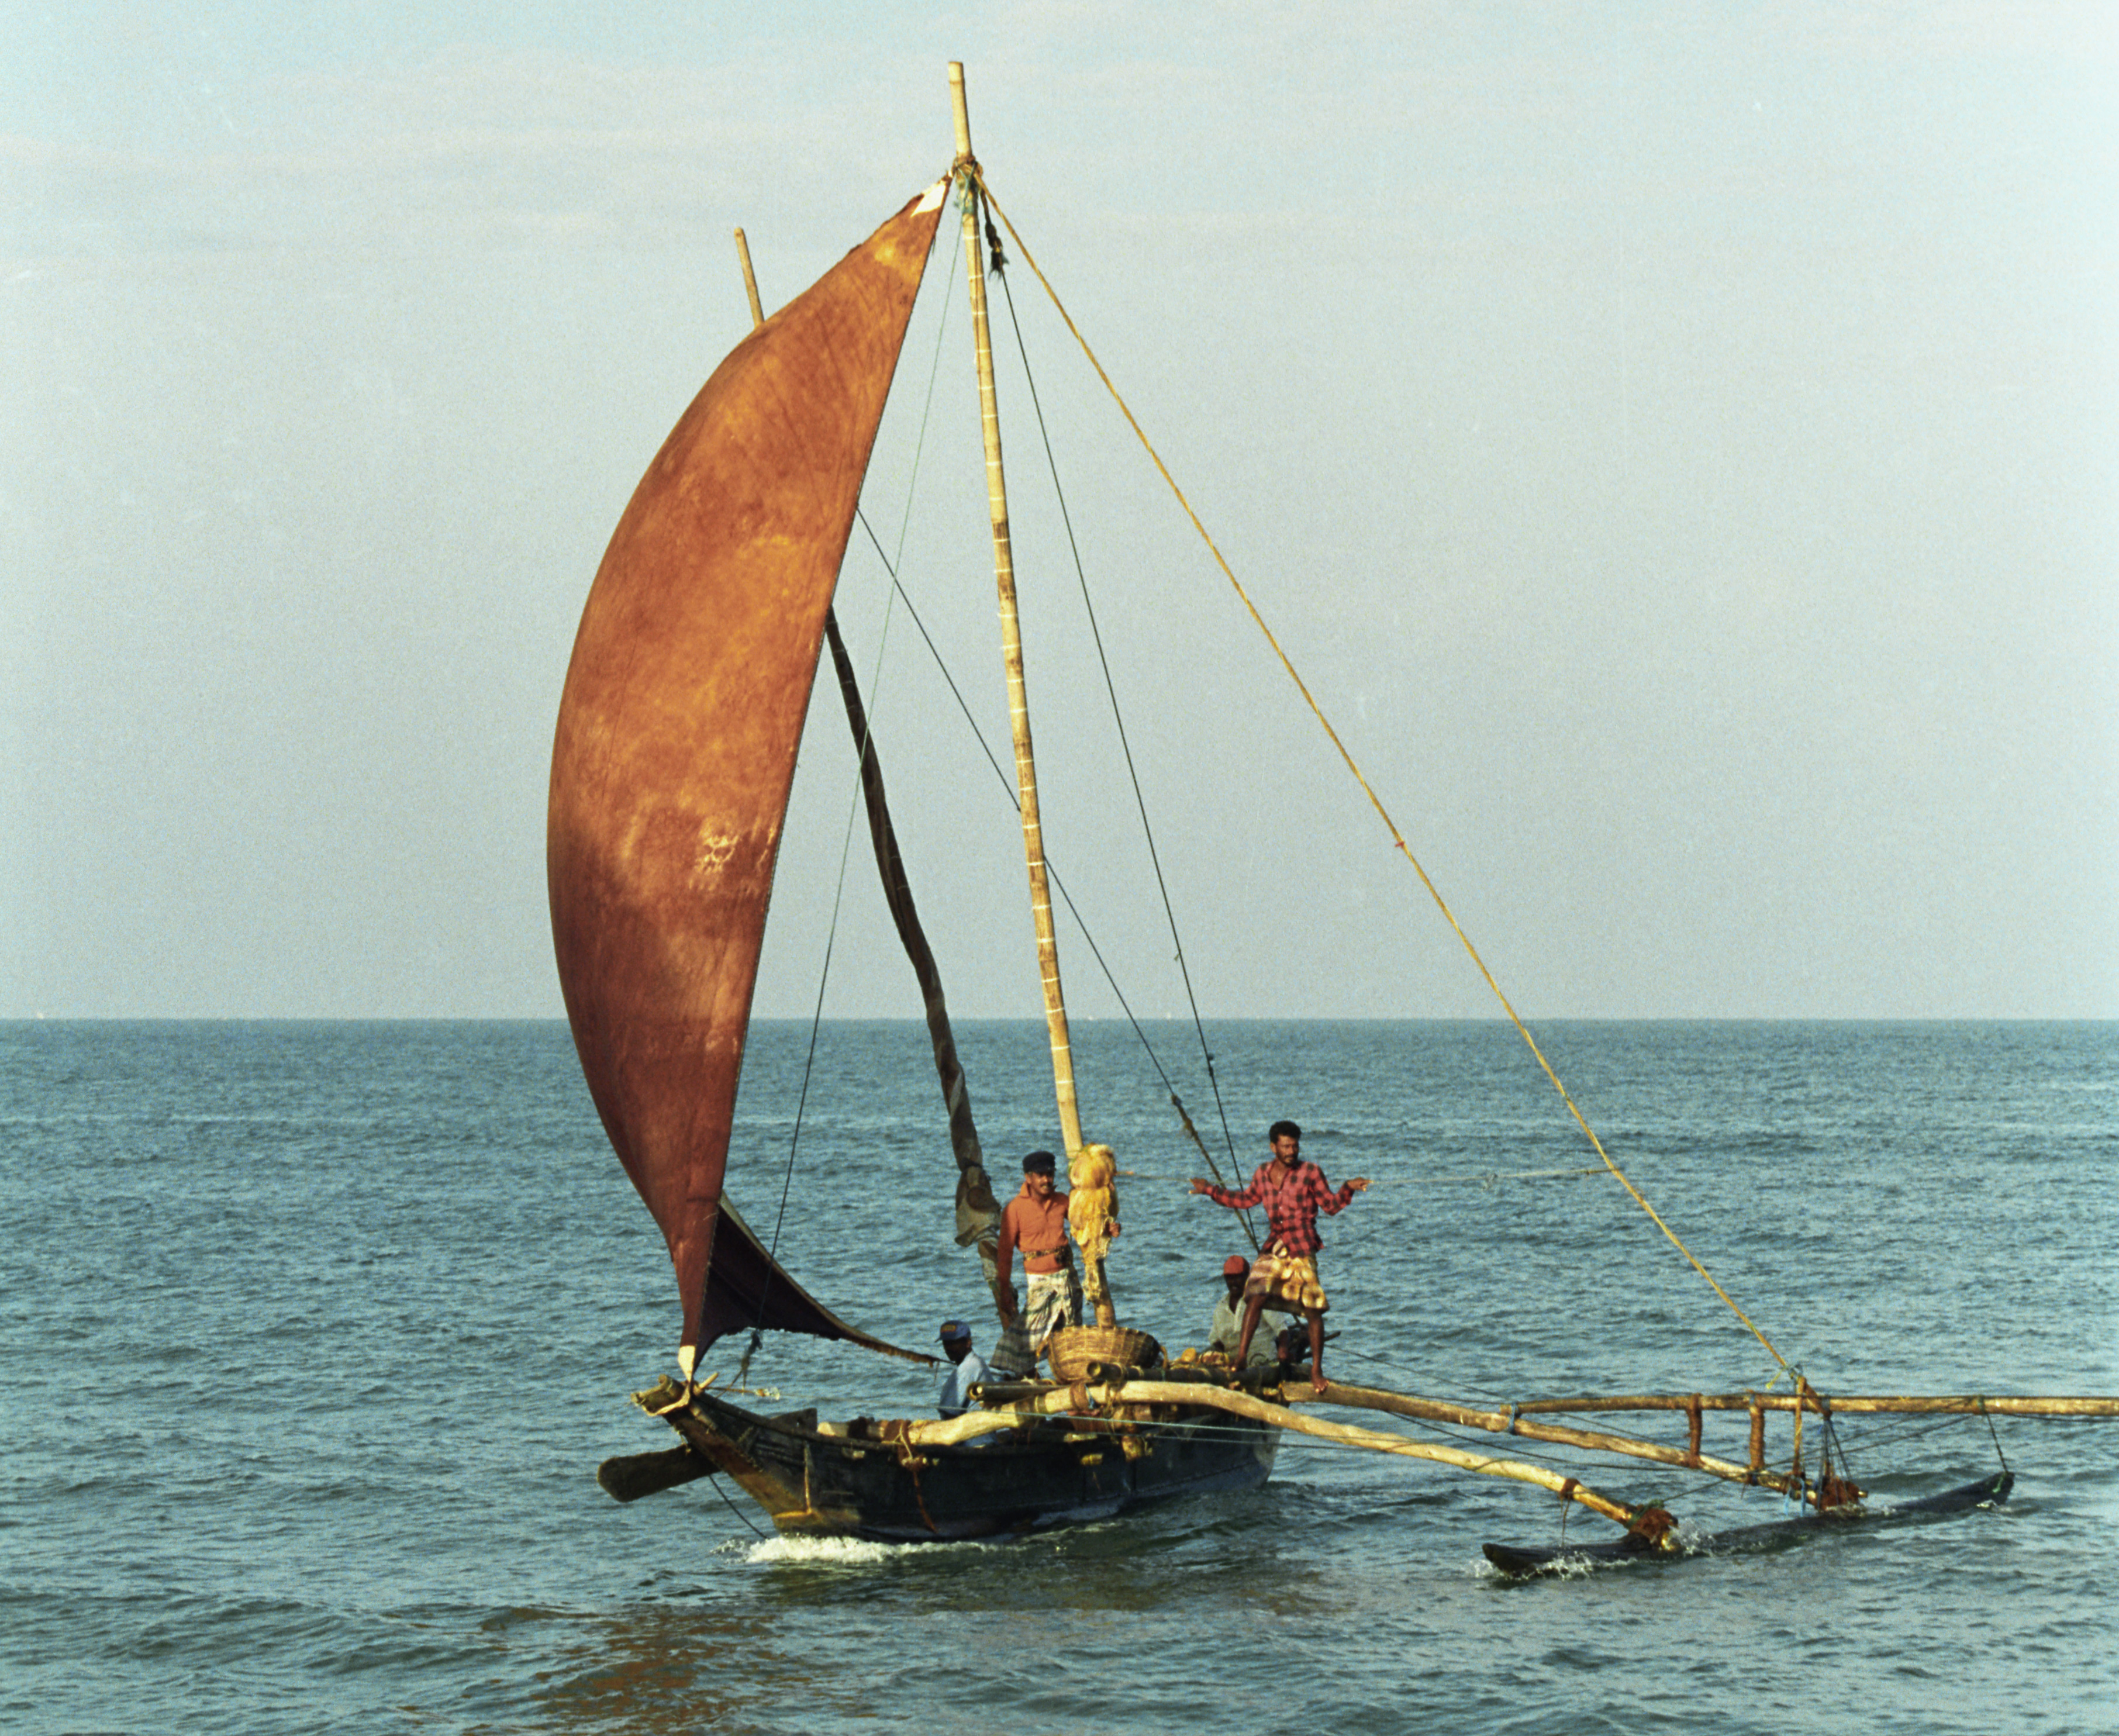
\includegraphics[width=\linewidth,height=1.75in,keepaspectratio=false]{figs/photo1.jpg}\par\vspace{2pt}
  \figcap{Outrigger fishing boat under a low-cost sail, Bay of Bengal (Sri Lanka). Photo: J.~Strzelecki, CC~BY~3.0.}
\end{minipage}
\par\vspace{6pt}
\begin{tcbraster}[raster columns=3, raster equal height, raster column skip=4mm]
 \begin{tile}{\fontsize{40}{42}\selectfont\bfseries\color{tg}1.2 bn L}\\[1pt]{\smallish diesel burnt each year by India's fishing fleet (ICAR-CIFT)}\end{tile}
 \begin{tile}{\fontsize{40}{42}\selectfont\bfseries\color{tg}56--77\,\%}\\[1pt]{\smallish of a boat's operating cost is spent on fuel (IISD, 2022)}\end{tile}
 \begin{tile}{\fontsize{40}{42}\selectfont\bfseries\color{acc}₹97→121}\\[1pt]{\smallish marine diesel per litre, Andhra Pradesh (press, 2026)}\end{tile}
\end{tcbraster}
\par\vspace{5pt}
\textbf{Research question:} \emph{can a low-cost sail plus a forecast-driven advisor deliver real, safe and bankable fuel savings for Indian small craft, and where and when do they pay?}
\end{secbox}
\vspace{\gap}
% ---------------- 2. IDEA & NOVELTY ----------------
\begin{secbox}{Our Solution: VaayuMitra (``Friend of the Wind'')}
{\centering
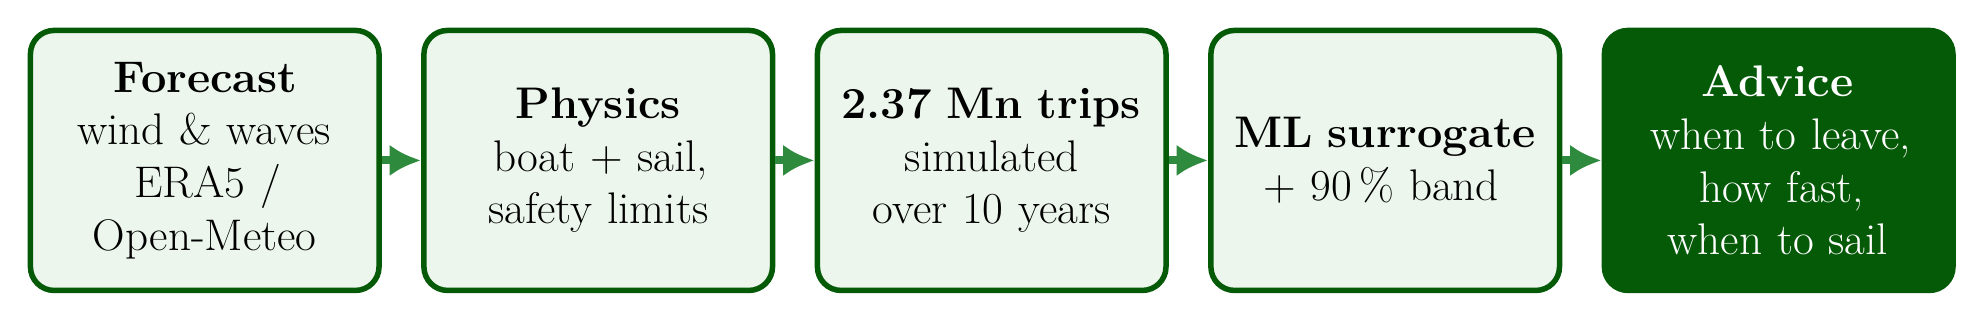
\begin{tikzpicture}[node distance=5mm, every node/.style={font=\fontsize{16}{19}\selectfont}]
  \tikzset{st/.style={draw=tg, line width=0.7mm, rounded corners=3mm, fill=lg, align=center,
                      minimum height=1.3in, text width=1.66in, inner sep=3pt}}
  \node[st] (a) {\textbf{Forecast}\\ wind \& waves\\ ERA5 / Open-Meteo};
  \node[st, right=of a] (b) {\textbf{Physics}\\ boat + sail,\\ safety limits};
  \node[st, right=of b] (c) {\textbf{2.37 Mn trips}\\ simulated\\ over 10 years};
  \node[st, right=of c] (d) {\textbf{ML surrogate}\\ + 90\,\% band};
  \node[st, right=of d, fill=tg, text=white] (e) {\textbf{Advice}\\ when to leave,\\ how fast, when to sail};
  \foreach \u/\v in {a/b,b/c,c/d,d/e} \draw[-{Latex[length=4mm,width=4mm]}, line width=1.0mm, mg] (\u) -- (\v);
\end{tikzpicture}\par}
\vspace{6pt}
\begin{minipage}[t]{0.6\linewidth}\vspace{0pt}
\textbf{What is new}
\begin{itemize}
  \item \hl{Retrofit + advisor}: a ₹12k soft sail on an existing FRP boat, plus a phone app that says \emph{when} the sail pays.
  \item \gb{Decade-long and coast-wide}: 10 years of hourly weather at {\NCell} sites along India's coast.
  \item Physics \gb{calibrated to measured Indian fuel rates} [3], with heel and sea-state \gb{safety limits}.
  \item \gb{Instant, honest ML}: a surrogate with calibrated uncertainty, explained by SHAP.
  \item \gb{Like-for-like validation} against fuel savings measured in real sail trials.
\end{itemize}
\end{minipage}\hfill
\begin{minipage}[t]{0.365\linewidth}\vspace{4pt}
  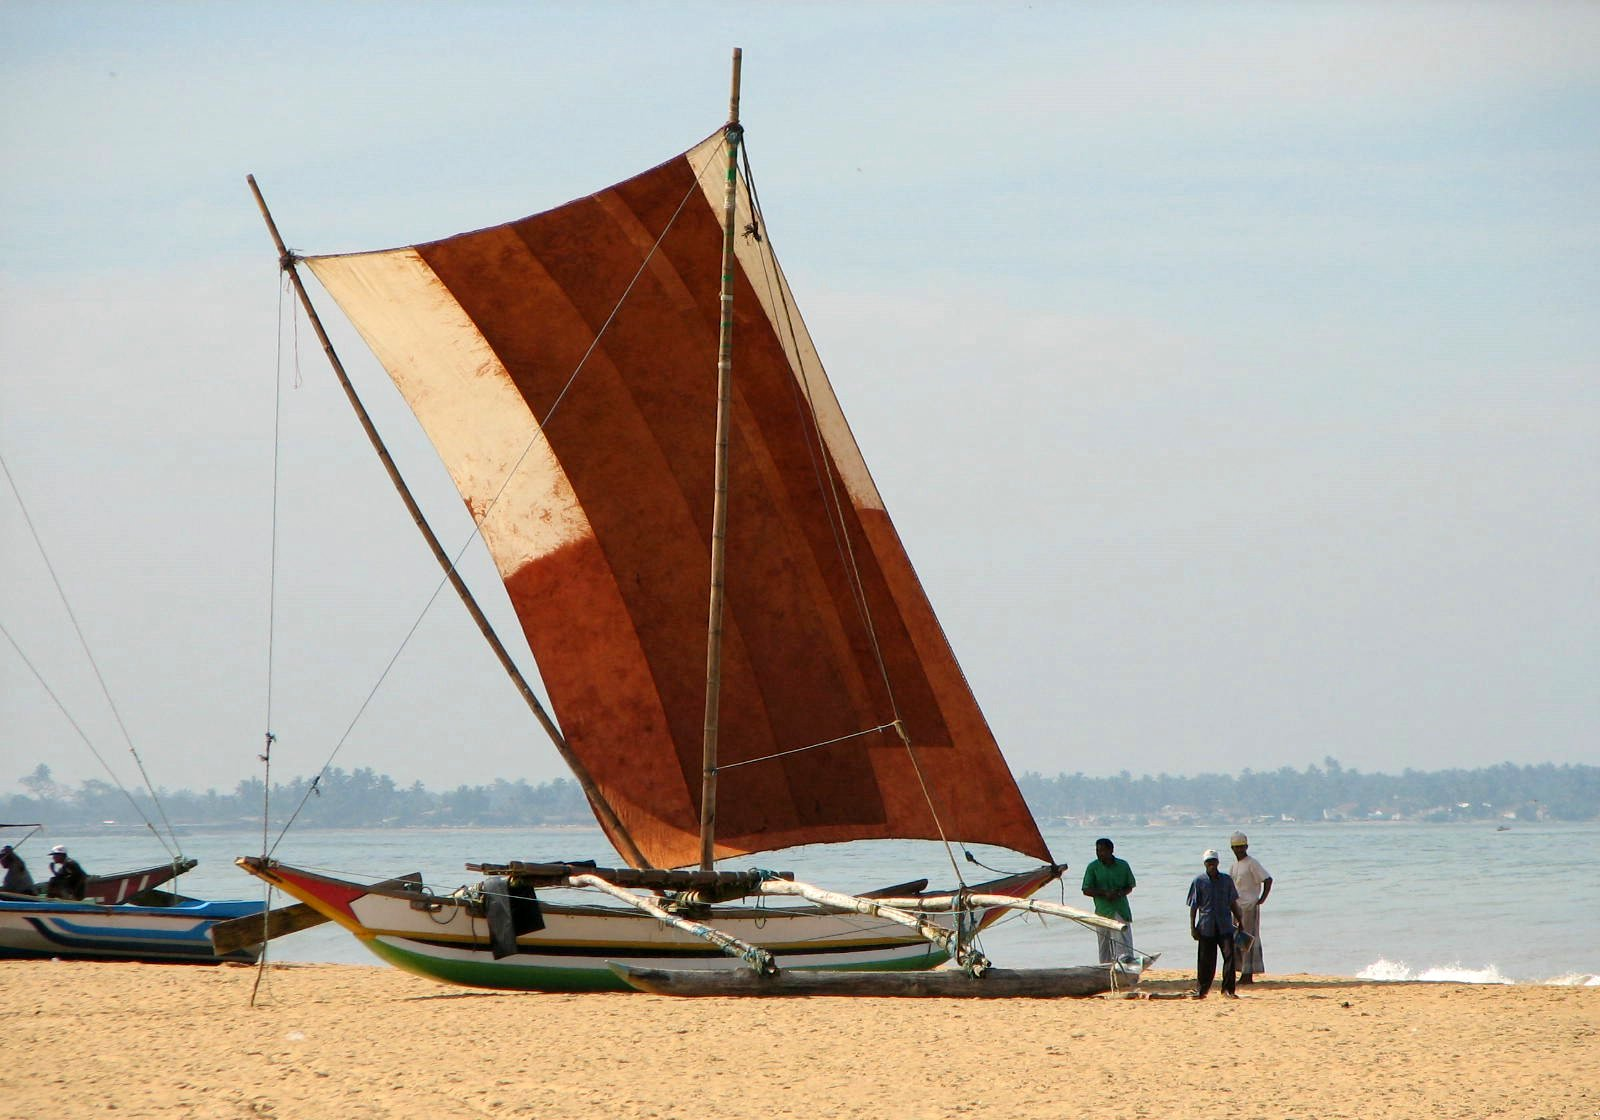
\includegraphics[width=\linewidth,height=1.6in,keepaspectratio=false]{figs/photo2.jpg}\par\vspace{2pt}
  \figcap{The kind of simple soft rig we retrofit: oruwa with its sail raised. Photo: B.~Gagnon, CC~BY-SA~3.0.}
\end{minipage}
\end{secbox}
\vspace{\gap}
% ---------------- 3. METHOD ----------------
\begin{secbox}{Methodology}
\begin{minipage}[t]{0.57\linewidth}\vspace{0pt}
\textbf{Sail forces} (lifting line, best trim every hour):
\begin{align*}
 F_x &= qA\,(C_L\sin\beta - C_D\cos\beta),\quad q=\tfrac12\rho_a V_A^2\\
 F_y &= qA\,(C_L\cos\beta + C_D\sin\beta),\quad C_D=C_{D0}+\tfrac{C_L^2}{\pi e\,AR}
\end{align*}
\textbf{Safety:} reef so that $F_y h_{CE}\le\Delta g\,GM\sin 8^\circ$; furl the sail if $H_s>2.5$\,m or $U_{10}>14$\,m/s.\\[3pt]
\textbf{Fuel} (Willans line calibrated to CIFT trials [3]; $R\propto V^{2.3}$; wave added resistance $R_{aw}$):
\begin{align*}
 \dot m &= m_0 + kP,\quad P=\big(R+R_{aw}-F_{\mathrm{net}}\big)\,V/\eta_D\\
 F_{\mathrm{net}} &= \max_{\alpha,\,r}\,(F_x-D_i),\quad D_i=\frac{F_y^2}{\tfrac12\rho_w V^2\pi s^2 e_h}
\end{align*}
\end{minipage}\hfill
\begin{minipage}[t]{0.41\linewidth}\vspace{0pt}\centering
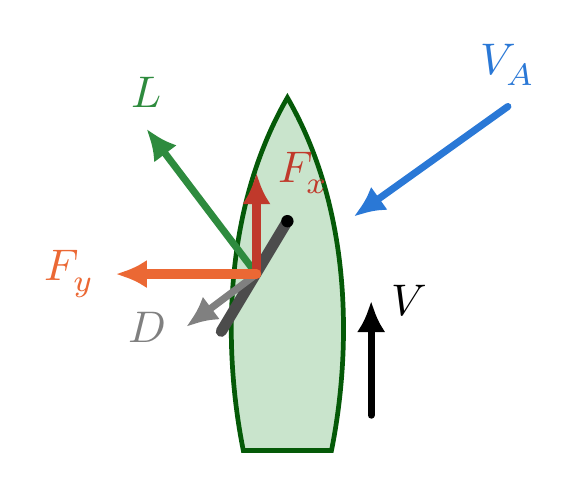
\begin{tikzpicture}[scale=1.12, line cap=round, >={Latex[length=4mm,width=3.6mm]},
                    every node/.style={font=\fontsize{16}{19}\selectfont}]
  \fill[lg2, draw=tg, line width=0.6mm] (0,2.3) .. controls (0.75,1.0) and (0.72,-0.6) .. (0.5,-1.7)
        -- (-0.5,-1.7) .. controls (-0.72,-0.6) and (-0.75,1.0) .. (0,2.3) -- cycle;
  \draw[line width=1.4mm, black!70] (0,0.9) -- (-0.75,-0.35);
  \fill (0,0.9) circle (0.07);
  \draw[->, line width=0.9mm, cblue] (2.5,2.2) -- (0.75,0.95) node[pos=0, above]{$V_A$};
  \coordinate (ce) at (-0.35,0.3);
  \draw[->, line width=0.9mm, mg] (ce) -- ++(-1.25,1.65) node[above]{$L$};
  \draw[->, line width=0.9mm, gray] (ce) -- ++(-0.8,-0.6) node[left]{$D$};
  \draw[->, line width=1.2mm, acc] (ce) -- ++(0,1.15) node[right]{$F_x$};
  \draw[->, line width=1.2mm, corange] (ce) -- ++(-1.6,0) node[left]{$F_y$};
  \draw[->, line width=0.9mm] (0.95,-1.3) -- (0.95,0.0) node[right]{$V$};
\end{tikzpicture}\par
\figcap{Only the forward force $F_x$ saves fuel; the side force $F_y$ heels the boat. Apparent wind $\vec V_A=\vec V_T-\vec V_B$.}
\end{minipage}
\par\vspace{4pt}
\begin{itemize}
  \item \textbf{Data:} hourly ERA5 wind and waves, {\Span} [5] $\rightarrow$ \textbf{\NTrips} single-day trips (3 harbours, 9 routes, 4 departure hours, 2 boats, 2 sails, 6/7/8\,kn); live forecast from Open-Meteo.
  \item \textbf{ML:} 5-member neural-net ensemble (GPU) trained on $\le$2021, calibrated on 2022 and \hl{tested on unseen 2023--24}; split-conformal 90\,\% bands; SHAP.
\end{itemize}
\par\vspace*{\padL}
\end{secbox}
\end{minipage}}
\sbox{\rcol}{\begin{minipage}[t]{0.493\textwidth}\vspace{0pt}
% ---------------- 4. RESULTS ----------------
\begin{secbox}{Results: Wind Is a Free Fuel}
\begin{minipage}[t]{0.525\linewidth}\vspace{0pt}
 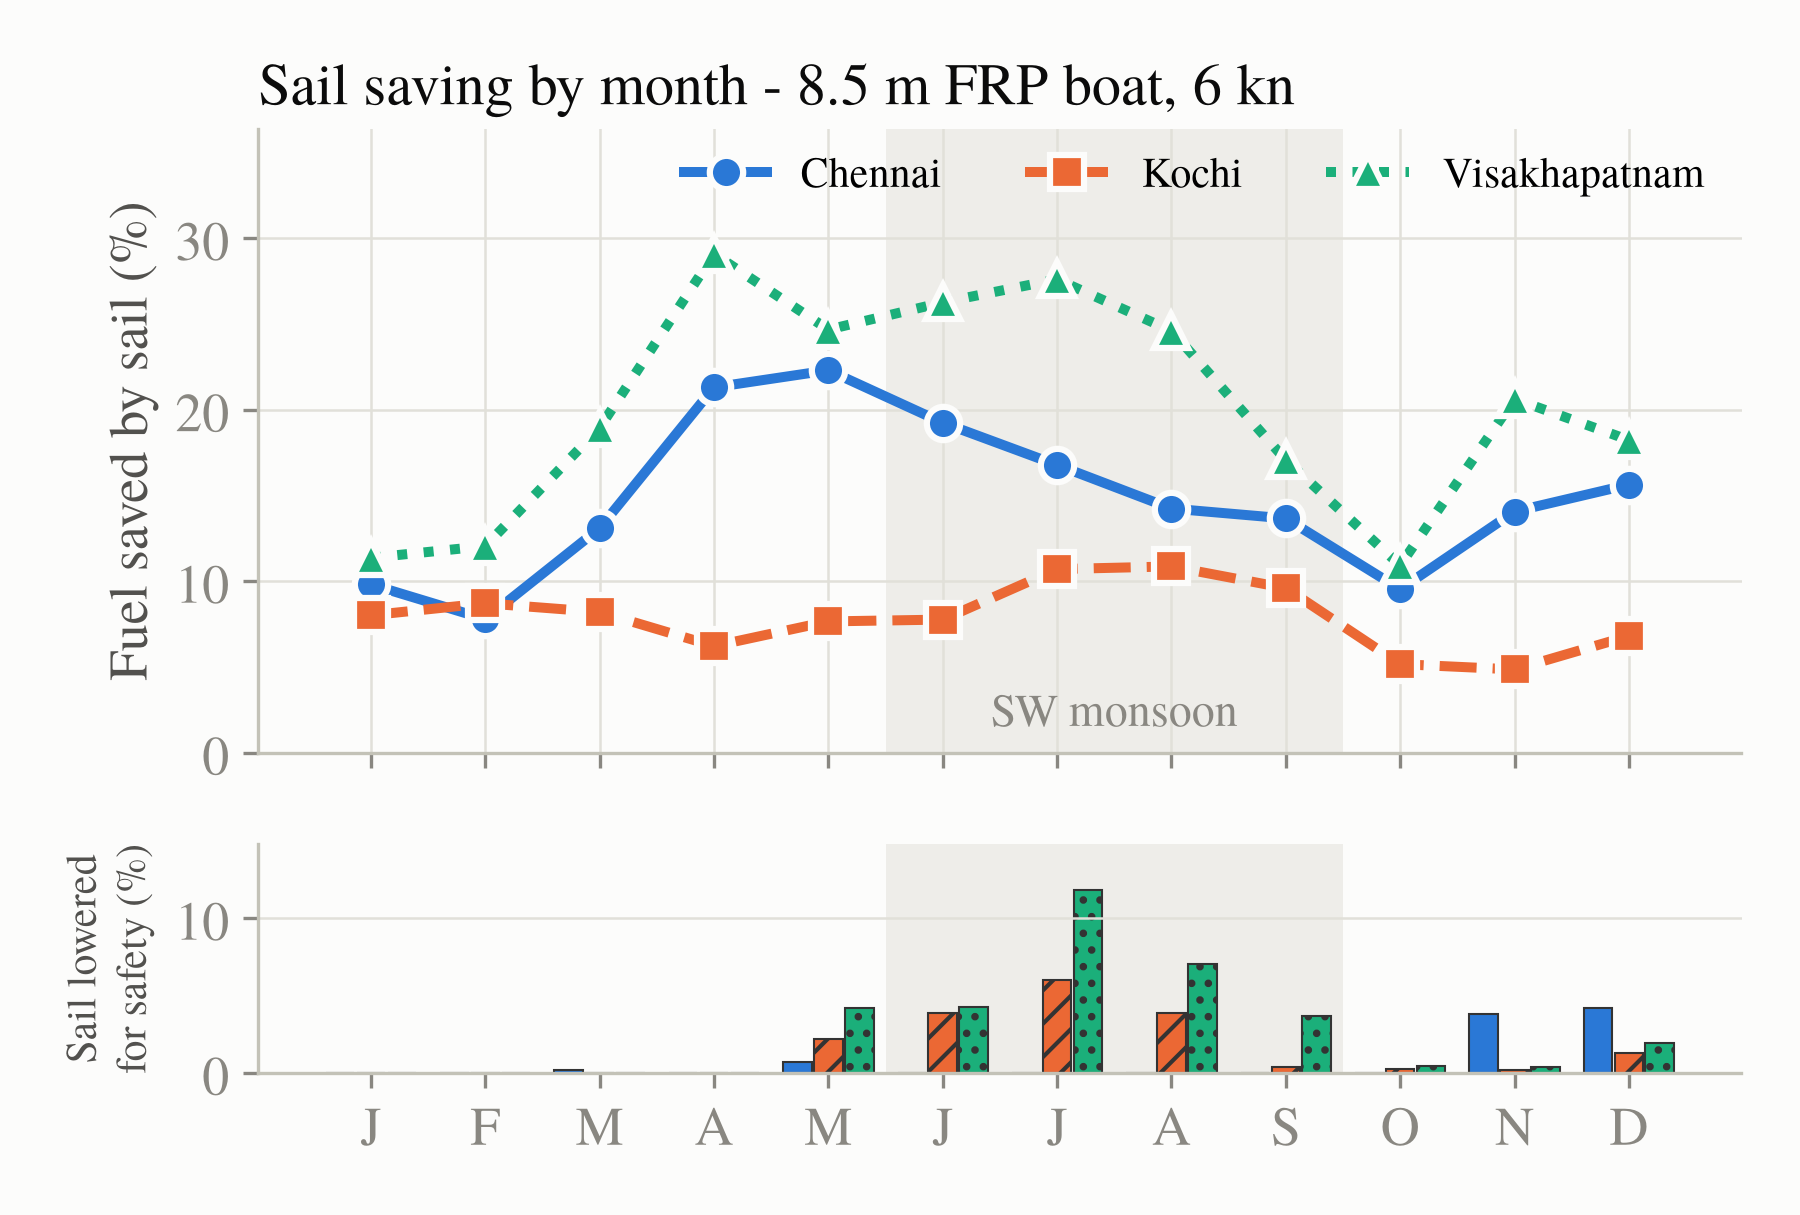
\includegraphics[width=\linewidth]{figs/F1_monthly_saving.png}\par
 \figcap{Monthly sail-only saving, FRP boat at 6\,kn (top); share of trips with the sail lowered for safety (bottom).}
\end{minipage}\hfill
\begin{minipage}[t]{0.445\linewidth}\vspace{0pt}
 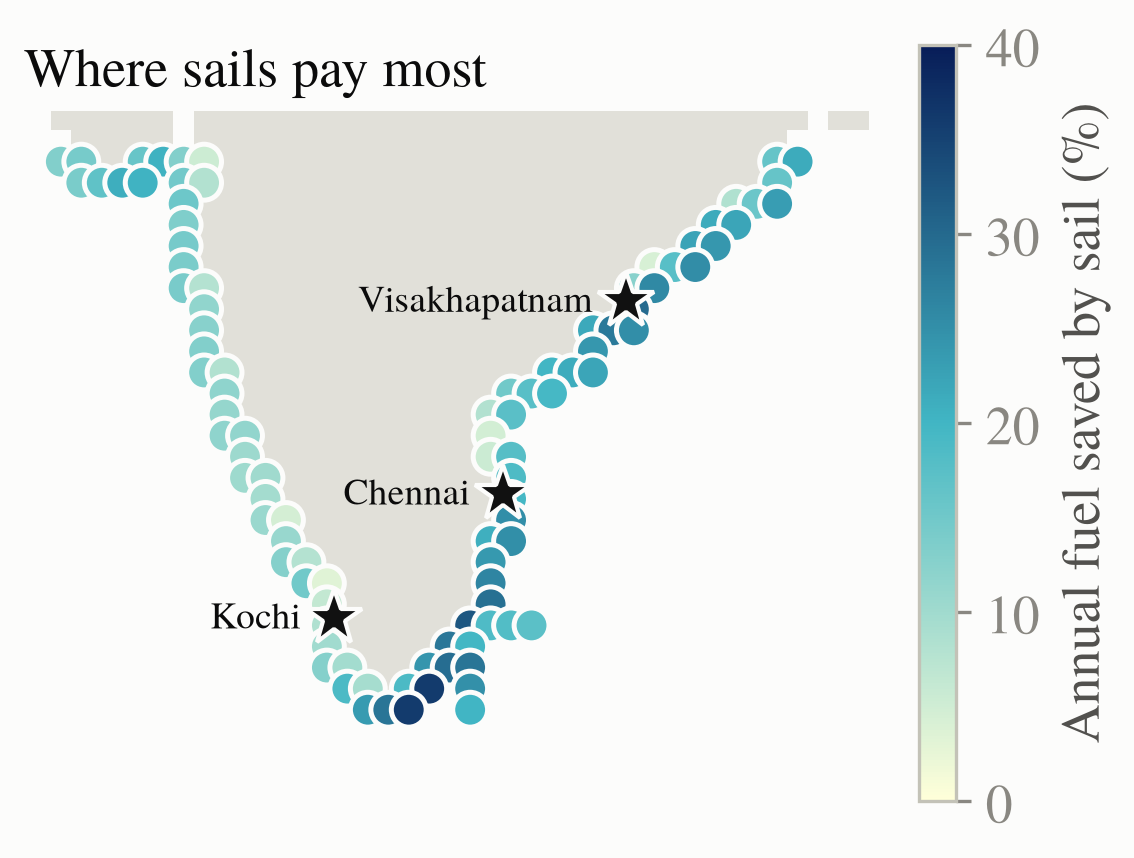
\includegraphics[width=\linewidth]{figs/F5_coast_map.png}\par
 \figcap{Annual sail-only saving at {\NCell} coastal sites along India, 2015--2024.}
\end{minipage}
\par\vspace{5pt}
\begin{minipage}[t]{0.5\linewidth}\vspace{0pt}
\begin{itemize}
  \item The sail alone saves \hl{\Kochi--\Vizag\,\%} of an FRP boat's diesel at 6\,kn (Kochi, Chennai, Visakhapatnam), up to \textbf{\BestPct\,\%} in \BestMonth.
  \item \gb{East coast} {\East}\,\% vs west coast {\West}\,\%; the Tamil Nadu tip reaches {\Tip}\,\%.
  \item \textbf{April--August} is the best season, while rough July seas force the sail down.
  \item \textbf{Slow + sail:} {\PkgBefore}\,→\,{\PkgAfter}\,L per trip (\hl{$-$\PkgPct\,\%}).
  \item \textbf{Stable:} results for 2015--19 and 2020--24 agree within 1\,\%.
\end{itemize}
\end{minipage}\hfill
\begin{minipage}[t]{0.44\linewidth}\vspace{0pt}
 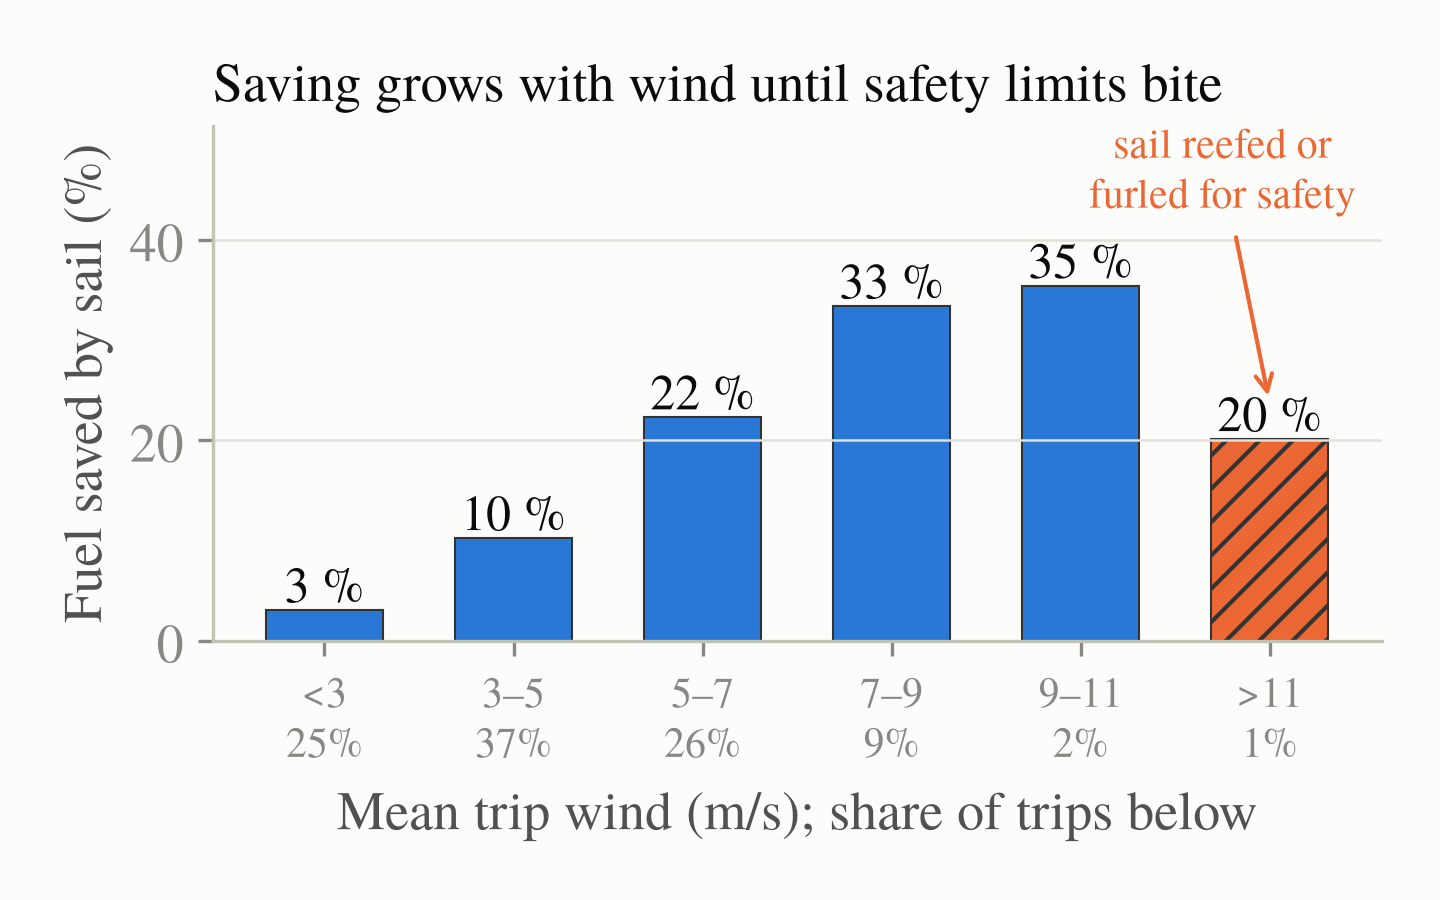
\includegraphics[width=0.9\linewidth]{figs/F7_wind_bins.png}\par
 \figcap{Saving against mean trip wind: it rises to 35\,\%, then safety reefing caps it.}
\end{minipage}
\end{secbox}
\vspace{\gap}
% ---------------- 5. ML ADVISOR + LIVE EXAMPLE ----------------
\begin{secbox}{Trustworthy ML Advisor}
\begin{minipage}[t]{0.44\linewidth}\vspace{0pt}
 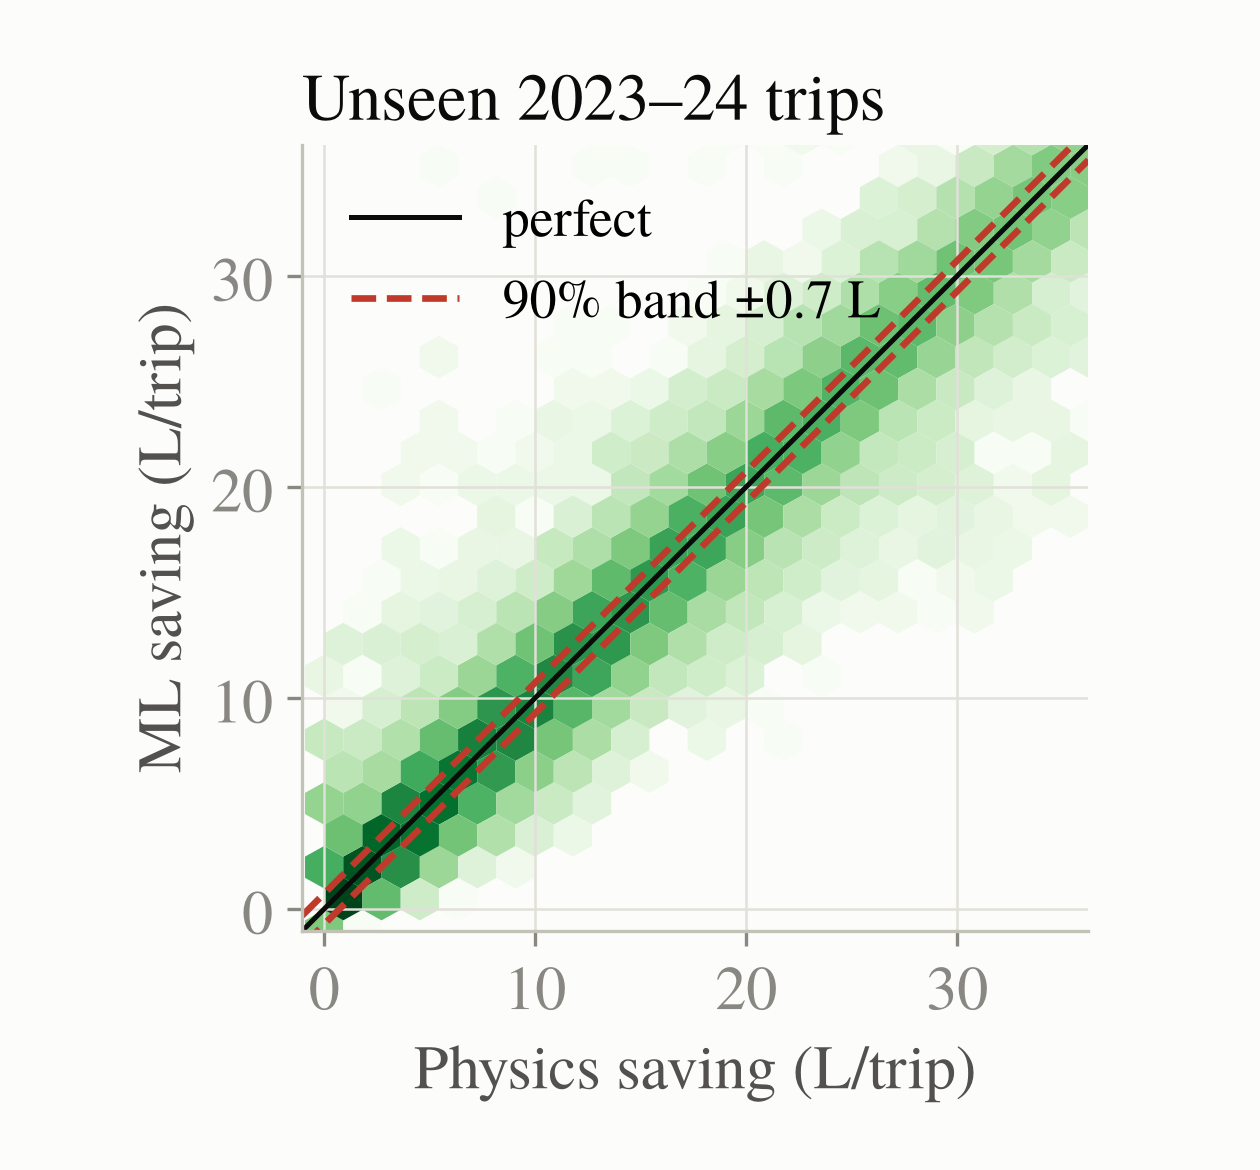
\includegraphics[width=\linewidth]{figs/F4b_parity.png}\par
 \figcap{Surrogate against physics on unseen trips; dashed: 90\,\% band.}
\end{minipage}\hfill
\begin{minipage}[t]{0.54\linewidth}\vspace{0pt}
 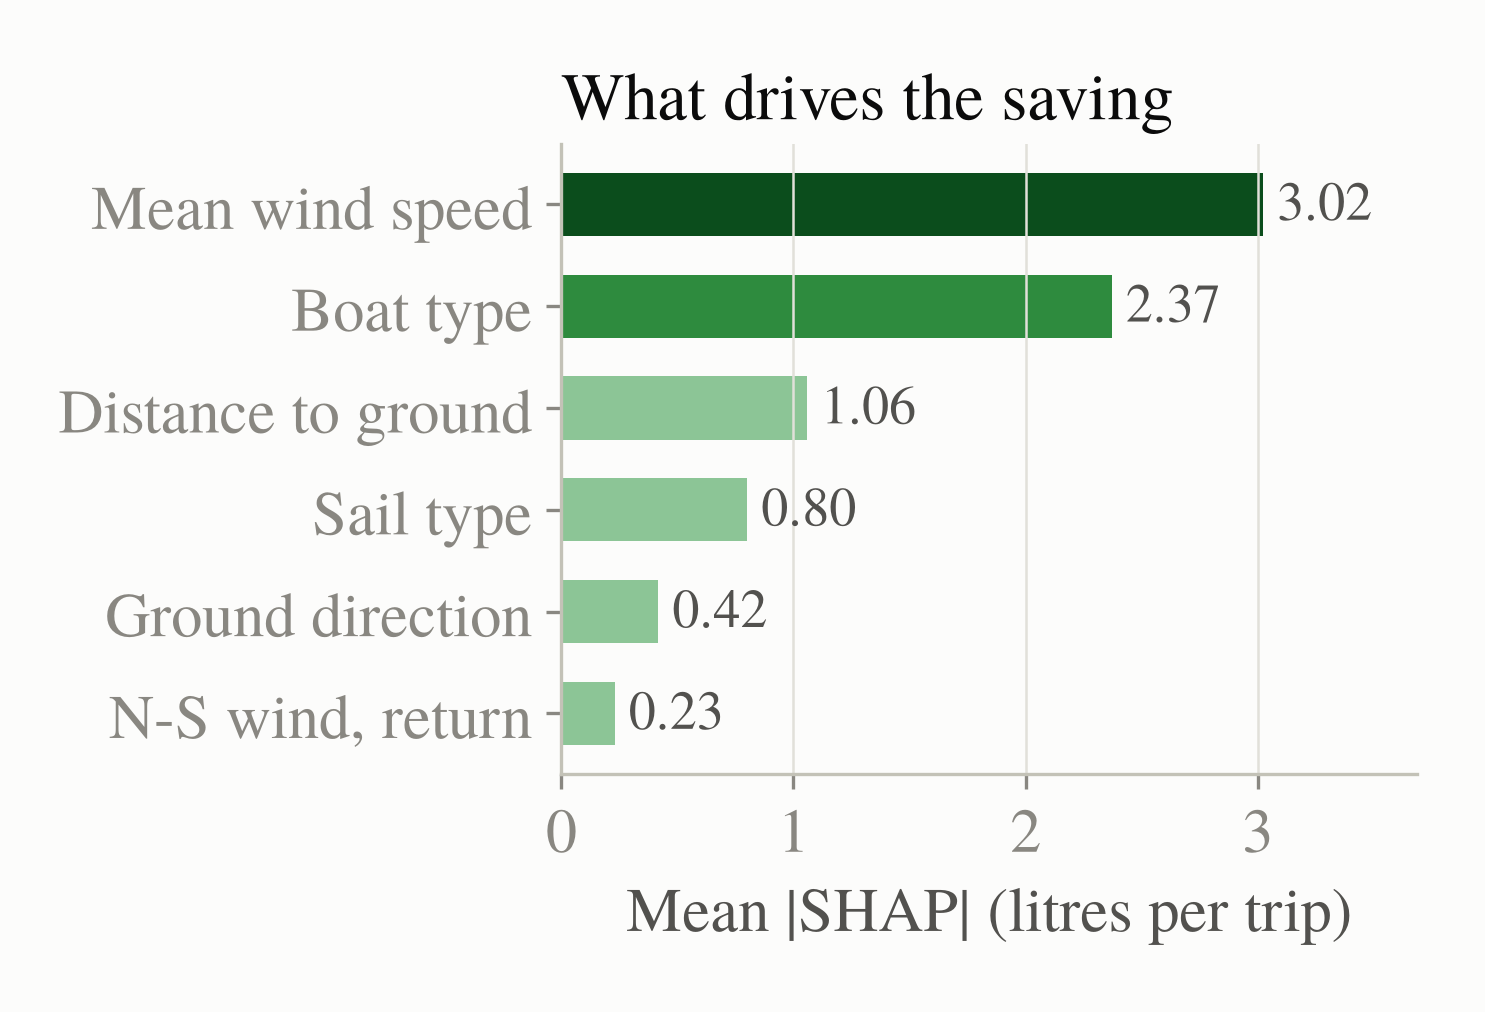
\includegraphics[width=\linewidth]{figs/F3b_shap.png}\par
 \figcap{SHAP: wind strength and boat type drive the saving.}
\end{minipage}
\par\vspace{10pt}
\begin{itemize}
  \item \hl{R$^2$ = \Rsq}, error \MAE\,L per trip (beats LightGBM); the \textbf{$\pm$\Qband\,L} band held on \textbf{\Cover\,\%} of test trips.
\end{itemize}
\vspace{12pt}
\begin{minipage}[t]{0.54\linewidth}\vspace{0pt}
 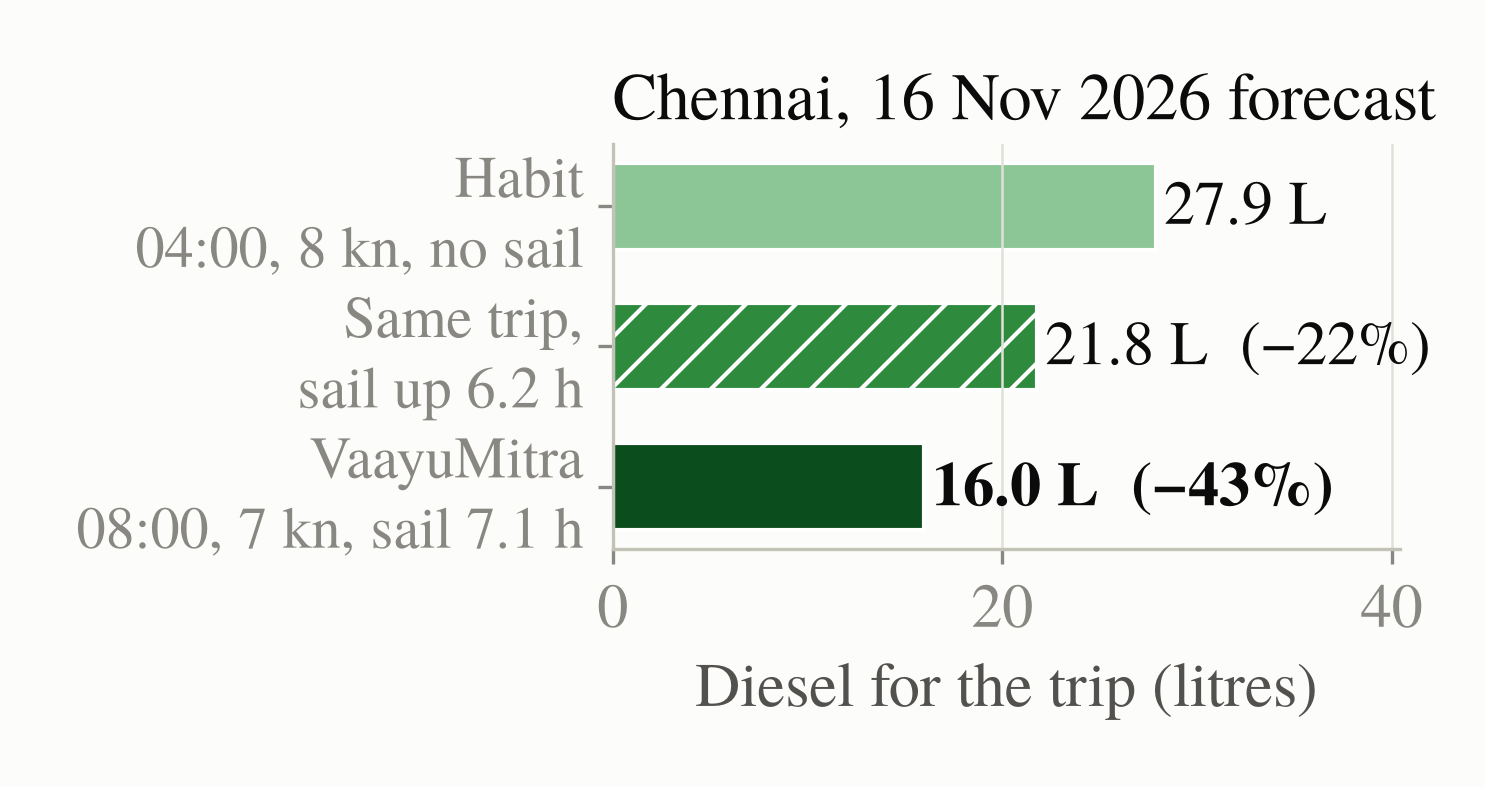
\includegraphics[width=0.92\linewidth]{figs/F9_live_plan.png}\par
 \figcap{Live advice, Chennai FRP boat, {\LiveDay}.}
\end{minipage}\hfill
\begin{minipage}[t]{0.43\linewidth}\vspace{0pt}
\textbf{A real day:} leaving at \BestDep\ at {\BestSpeed}\,kn with the sail up {\BestSail}\,h saves \hl{\BestSavePct\,\% diesel} (₹\BestSaveRs) for one hour more at sea.\par\vspace{6pt}
\begin{minipage}[c]{0.46\linewidth}
\includegraphics[width=\linewidth]{figs/qr_app.png}\end{minipage}\hfill
\begin{minipage}[c]{0.5\linewidth}{\smallish\raggedright\textbf{Scan to try it} on any phone: live forecast, English or Tamil\par}\end{minipage}
\end{minipage}
\par\vspace*{\padR}
\end{secbox}
\end{minipage}}
\typeout{COLS: L=\the\dimexpr\ht\lcol+\dp\lcol\relax\space R=\the\dimexpr\ht\rcol+\dp\rcol\relax}
\usebox{\lcol}\hfill\usebox{\rcol}

\vspace{\gap}
% =====================================================================
%  IMPACT (full width)
% =====================================================================
\begin{secbox}{Impact: Per Boat and at National Scale \quad{\fontsize{20}{24}\selectfont\mdseries(SDG 7 · 13 · 14)}}
\begin{tcbraster}[raster columns=5, raster equal height, raster column skip=5mm]
 \begin{tile}{\fontsize{34}{37}\selectfont\bfseries\color{tg}\Payback\ months}\\[3pt]{\smallish payback of a ₹12k sail}\end{tile}
 \begin{tile}{\fontsize{34}{37}\selectfont\bfseries\color{tg}₹\InrBoat k}\\[3pt]{\smallish saved per boat a year (₹\LakhPkg\,lakh if slowed)}\end{tile}
 \begin{tile}{\fontsize{34}{37}\selectfont\bfseries\color{tg}\MLdiesel\ Mn L}\\[3pt]{\smallish diesel saved a year, all India [4]}\end{tile}
 \begin{tile}{\fontsize{34}{37}\selectfont\bfseries\color{tg}₹\Crore\ cr}\\[3pt]{\smallish saved a year by \Craft\ boats [4]}\end{tile}
 \begin{tile}{\fontsize{34}{37}\selectfont\bfseries\color{tg}\Ktco\ kt}\\[3pt]{\smallish CO$_2$ avoided a year, all India [4]}\end{tile}
\end{tcbraster}
\end{secbox}

\vspace{\gap}
% =====================================================================
%  BOTTOM ROW: feasibility | validation + next steps
% =====================================================================
\newsavebox{\lstack}\newlength{\lstackH}
\sbox{\lstack}{\begin{minipage}[t]{0.493\textwidth}\vspace{0pt}
\begin{secbox}{Feasibility Study}
{\fontsize{16}{19}\selectfont
\renewcommand{\arraystretch}{1.04}
\begin{tabularx}{\linewidth}{@{}p{0.17\linewidth}>{\justifying\arraybackslash}X@{}}
 \gb{Technical} & The rig is proven: FAO/BOBP built and sailed it on Indian beach-landing boats [1]; sails are still used daily by Bay of Bengal fishers. No engine change. \\[2pt]
 \gb{Economic} & Payback is \textbf{\Payback\ months} as modelled, still \hl{\PayAtSix\ months at the 6\,\% saving measured in 1983 trials} (₹\InrAtSix k a year) and \textbf{\PayWorst\ months} if every assumption turns against us. \\[2pt]
 \gb{Operational} & Free forecast data, a basic phone or SMS, no new skills to decide; the sail is dropped while nets are worked. \\[2pt]
 \gb{Safety} & Heel kept below 8$^\circ$; the sail is furled in high wind or seas above 2.5\,m. \\[2pt]
 \gb{Scale-up} & Pilot with one Chennai cooperative, then State fisheries schemes; the app costs almost nothing per boat. \\[2pt]
\end{tabularx}\par}
\end{secbox}
\par\vspace{\gap}
\begin{secbox}{References}
\fontsize{13}{15.5}\selectfont\raggedright
[1] Gulbrandsen, Ø. (1984). Fishing craft development in Kerala. BOBP/WP/25, FAO.\par
[2] Rebel Marine Service (1983). Sails on fishing vessels. NMFS NA-80-FA-D-0012.\par
[3] ICAR-CIFT. Dual-fuel trawler trials off Kochi. \emph{Fishery Technology}, ICAR.\par
[4] ICAR-CMFRI (2020). Marine Fisheries Census 2016: India.\par
[5] Hersbach, H. et al. (2020). ERA5 reanalysis. \emph{QJRMS} 146, 1999--2049.\par
Photos: Wikimedia Commons, licences as credited.
\end{secbox}
\end{minipage}}
\setlength{\lstackH}{\ht\lstack}\addtolength{\lstackH}{\dp\lstack}
\noindent\usebox{\lstack}\hfill
\begin{minipage}[t][\lstackH][t]{0.493\textwidth}\vspace{0pt}
\begin{secbox}[height fill, valign=center]{Validation and Next Steps}
\begin{minipage}[c]{0.58\linewidth}
 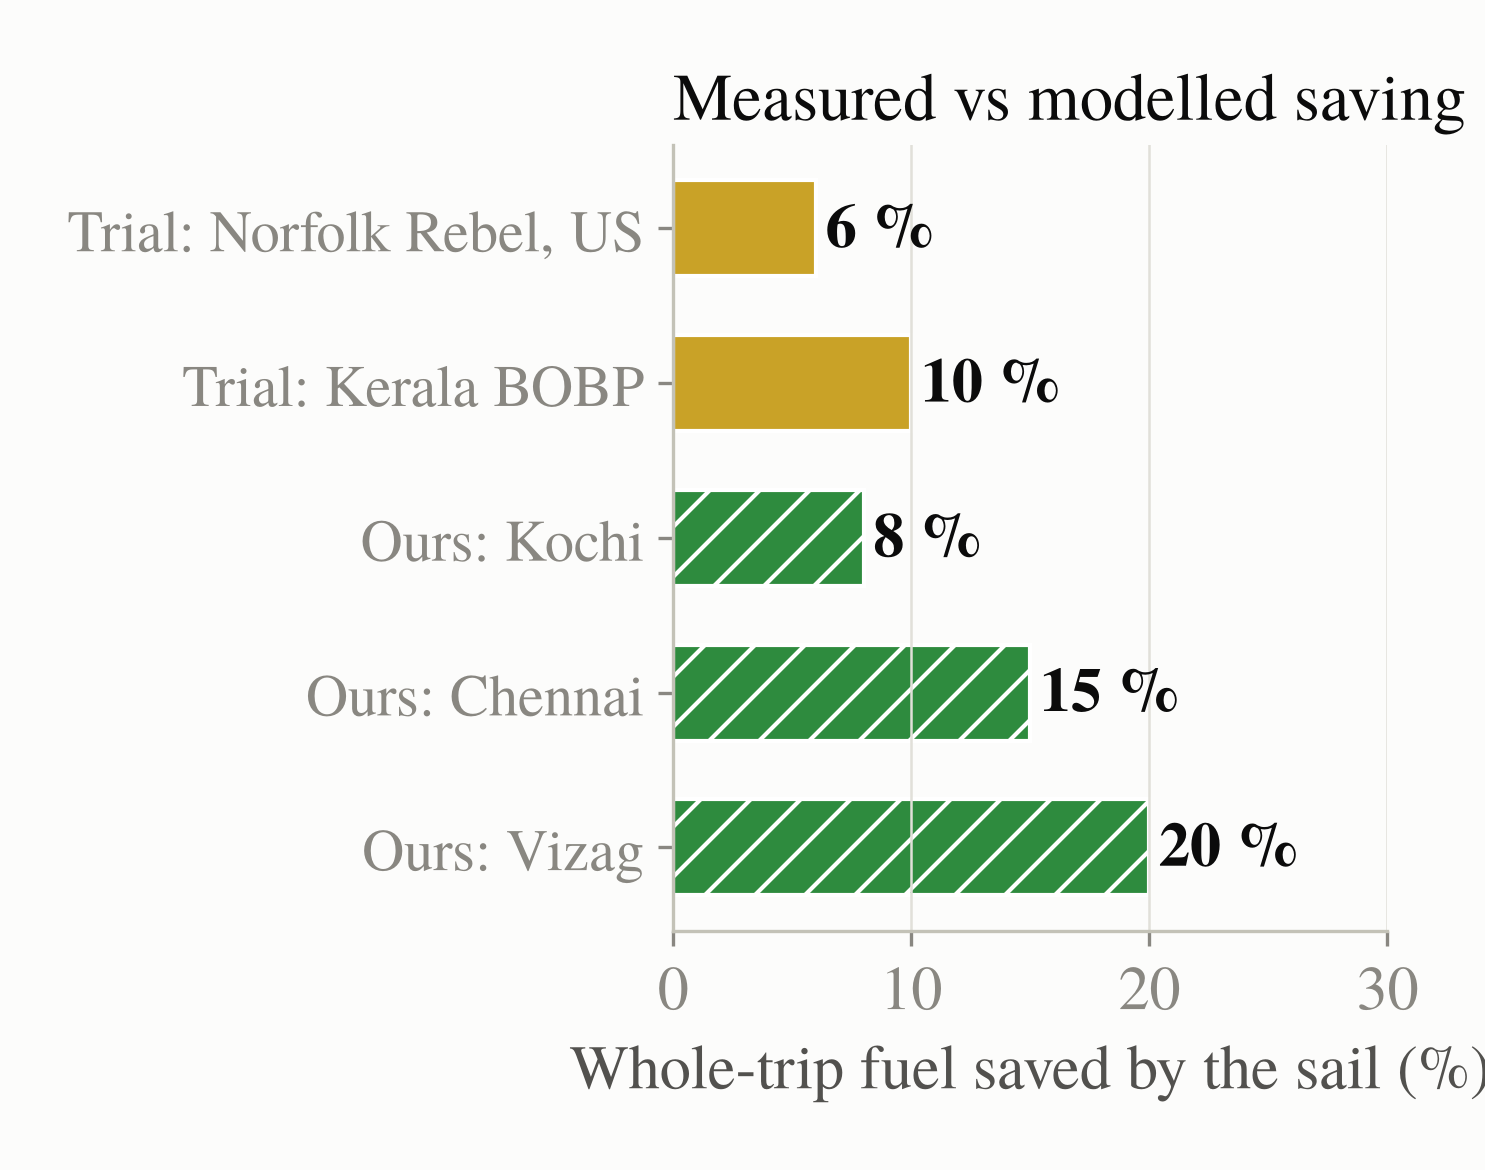
\includegraphics[width=\linewidth]{figs/F8b_validation.png}\par
 \figcap{Trial savings [1,2] against our model.}
\end{minipage}\hfill
\begin{minipage}[c]{0.39\linewidth}
\begin{itemize}
  \item Our {\Kochi}--{\Vizag}\,\% is a \textbf{technical potential}; real trials measured 6--10\,\%, which \hl{still pays back within a year}.
  \item \textbf{Robust:} payback stays at \PayMin--\PayMax\ months for $\pm$20\,\% changes in any physics or cost input.
  \item \textbf{Conservative:} for slow steaming our model gives $-$34\,\% fuel per nm; trials measured $-$51\,\%.
  \item \textbf{Next:} a logged sea trial on a Chennai FRP boat, and Tamil voice/SMS advice built with fishers.
\end{itemize}
\end{minipage}
\end{secbox}
\end{minipage}

\end{document}
